\newpage

\section{Architecture Diagram}
\subsection{Architectural Decision Rationale}
Architectural diagrams provide a structured view of how a software system is organized and how its components interact. In modern software development, two primary architectural styles are commonly considered: \textbf{monolithic architecture} and \textbf{microservice architecture}.

A \textbf{monolithic architecture} is a traditional model of a software program, which is built as a unified unit that is self-contained and independent from other applications. The word “monolith” is often attributed to something large and glacial, which isn’t far from the truth of a monolith architecture for software design. \cite{atlassian_microservices_vs_monolith}

A \textbf{microservices architecture}, also simply known as microservices, is an architectural method that relies on a series of independently deployable services. These services have their own business logic and database with a specific goal. Updating, testing, deployment, and scaling occur within each service. Microservices decouple major business, domain-specific concerns into separate, independent code bases. \cite{atlassian_microservices_vs_monolith}

As can be seen, the choice between these architectural approaches depends on the project’s specific requirements, team size, and long-term goals. Smaller systems or teams often benefit from the straightforwardness of monolithic architecture, while larger, more complex systems may require the flexibility and scalability of distributed services.

After evaluating our project goals and team size, we decided to implement a service-based modular monolith as the core architectural foundation for CodeRank. The key reasons for selecting this approach include:
\begin{itemize}
    \item \textbf{Team Size and Feasibility}
With only two members, adopting a full microservice architecture would introduce significant overhead in DevOps, deployment, and service management. In contrast, a modular monolith allows us to focus on implementing core features without the burden of distributed complexity.
    \item \textbf{Easier Development and Maintenance}
By separating the system into modules—such as the Discussion Module, Submission Module, Auth Module, and Contest Module—we can maintain clean boundaries within a single codebase. This structure enables faster development cycles and reduces merging conflicts.
    \item \textbf{Future Scalability}
While CodeRank currently operates as a monolithic application, its modules are designed following \textbf{Domain-Driven Design} (DDD) principles. These boundaries can later be extracted into microservices if the system needs to scale. This ensures long-term flexibility without requiring microservices prematurely.
\end{itemize}
\begin{figure}[h!]
    \centering
    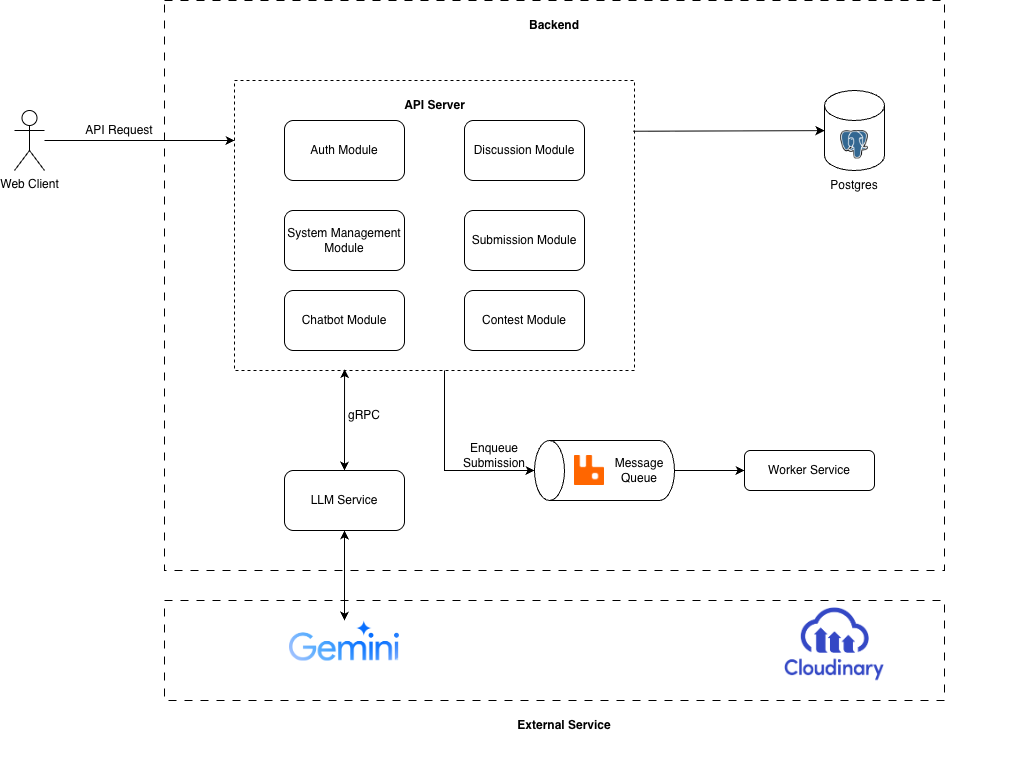
\includegraphics[width=1\textwidth]{Contents/Chapter 3/Architecture Diagram/CodeRank.drawio.png}
    \vspace{0.6cm}
    \caption{Architecture Diagram}
    \label{fig:leetcode-system}
\end{figure}
\clearpage

\subsection{System Components}

\begin{figure}[h!]
    \centering
    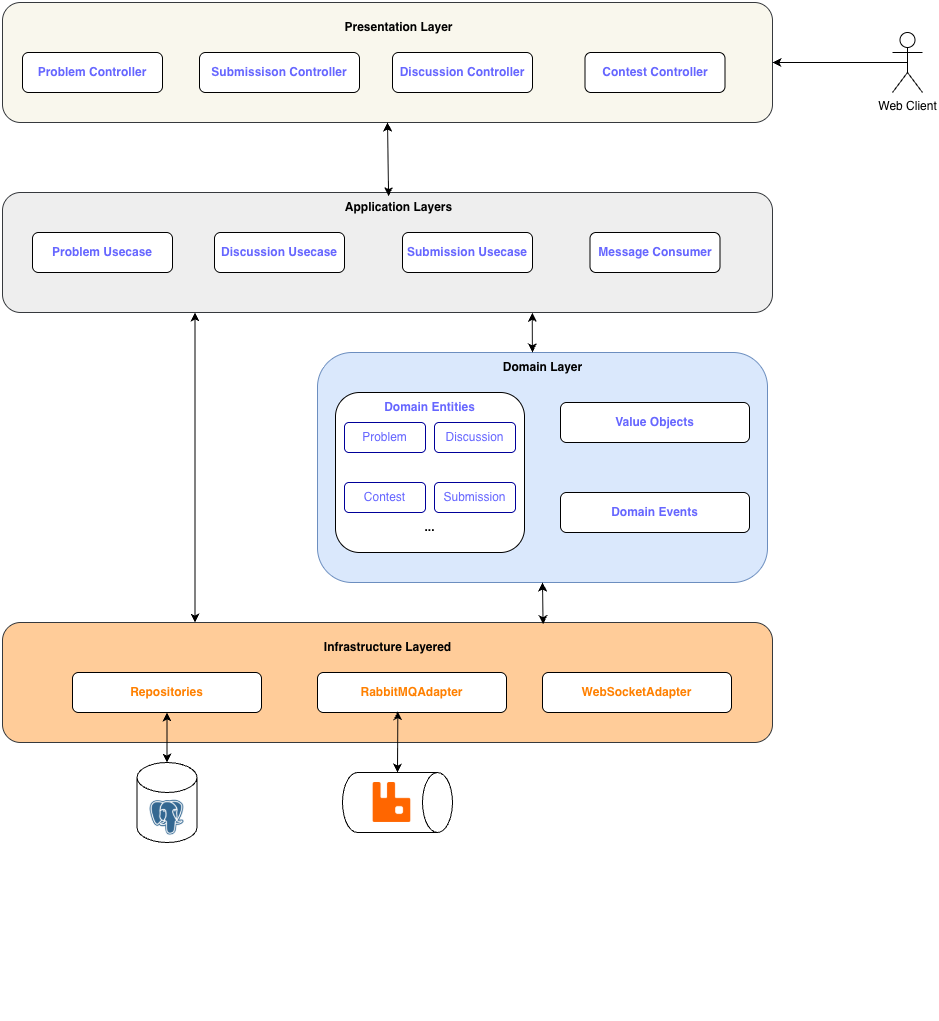
\includegraphics[width=1\textwidth]{Contents/Chapter 3/Architecture Diagram/LayeredArchitecture.drawio.png}
    \vspace{0.6cm}
    \caption{Layered Architecture}
    \label{fig:leetcode-system}
\end{figure}
The system architecture of CodeRank is organized into four primary layers, each responsible for a specific set of functions. This layered approach ensures clean separation of concerns, maintainability, and a clear mapping between business rules and system implementation.

\begin{enumerate}
  \item \textbf{Presentation Layer}
  
The \textbf{Presentation Layer} acts as the entry point for all external interactions with the system. It exposes various controllers such as the \textit{Problem Controller}, \textit{Submission Controller}, \textit{Discussion Controller}, and \textit{Contest Controller}, which handle incoming HTTP requests from the web client. These controllers validate user input, map requests to the appropriate application use cases, and return responses in a structured format. This layer focuses purely on communication and does not contain business logic, ensuring the interface remains thin and easily adaptable.
    \item  \textbf{Application Layer}
    
The \textbf{Application Layer} contains the system’s core orchestrators, known as Use Cases. Examples include the Problem Usecase, Discussion Usecase, Submission Usecase, and a dedicated Message Consumer for asynchronous tasks.

This layer coordinates operations between the Presentation Layer and the Domain Layer, ensuring that business rules are executed in the correct sequence. It does not implement business rules itself; instead, it acts as a mediator, invoking domain logic and triggering events. This design improves code clarity and supports future expansion.

    \item  \textbf{Domain Layer}
    
The \textbf{Domain Layer} represents the heart of the application, where all business logic and system rules are defined. It contains: 

\begin{itemize}
    \item Domain Entities such as Problem, Discussion, Contest, and Submission.
    \item Value Objects that encapsulate immutable attributes or concepts.
Domain Events used to capture and react to significant changes within the system.
    \item Domain Events used to capture and react to significant changes within the system.
\end{itemize}

    \item  \textbf{Infrastructure Layer}
    
The \textbf{Infrastructure Layer} provides the technical capabilities required to support the domain and application layers. It includes: 

\begin{itemize}
    \item \textbf{Repositories}, which manage communication with the PostgreSQL database.
    \item \textbf{RabbitMQ Adapters}, responsible for publishing and consuming messages for asynchronous processing.
Domain Events used to capture and react to significant changes within the system.
    \item \textbf{WebSocket Adapters}, enabling real-time communication such as live updates for submissions or discussion activities.
\end{itemize}

This layer abstracts external systems and framework-specific operations, ensuring that the upper layers remain decoupled from technical implementation details.

\end{enumerate}